\lab{Электромагнитные волны в волноводе} 

\begin{lab:aim} ознакомление с особенностями распространения
    электромагнитных волн в волноводе, аппаратурой и методами измерения основных
    характеристик протекающих при этом процессов. 
\end{lab:aim}

\begin{lab:equipment} генератор сигналов сверхвысокой частоты, измерительная
    линия, усилитель, заглушка, отрезок волновода с поглощающей нагрузкой, отрезки
    волноводов различных сечений, детекторная головка. 
\end{lab:equipment}

Передача энергии электромагнитных колебаний низкой частоты, например, 50~Гц, не
представляет проблем и делается широко известным способом: по проводам. На более
высоких частотах (до 300~МГц) эта задача решается с помощью двухпроводных линий
и коаксиальных кабелей. На ещё более высоких частотах (до 300~ГГц) при
колебаниях с длинами волн (в вакууме) от 1~м до 1~мм (этот диапазон
называется \important{диапазоном сверхвысоких частот} или, сокращённо, СВЧ)
передача энергии с помощью двухпроводной линии или коаксиальных кабелей
становится малоэффективной из-за больших потерь: резко возрастает сопротивление
проводов из-за \important{скин-эффекта}~--- вытеснения тока на поверхность, а в
двухпроводной линии, кроме того, потери растут вследствие излучения энергии в
окружающее пространство.

В СВЧ-диапазоне энергия передаётся с помощью металлических труб, называемых
волноводами (в миллиметровом диапазоне длин волн волноводы могут быть сделаны и
из диэлектрика). Электромагнитные волны могут распространяться по металлическим
трубам любого профиля, но из технологических соображений сечения волноводов
делаются либо круглыми, либо прямоугольными.

Чтобы найти структуру электромагнитного поля в волноводе, нужно решить \emph{волновое
уравнение} с соответствующими граничными условиями. Простейший пример такого решения,
относящийся к волноводу прямоугольного сечения с идеально проводящими стенками,
рассмотрен во Ведении к разделу.

Если в волноводе имеется препятствие или нерегулярность, распространяющаяся по оси
$z$ волна частично или полностью отражается от него. При сложении 
отражённой и падающей волн образуется \emph{стоячая волна} с узлами
и пучностями. Расстояние между узлами $\Delta z_m$ (или между пучностями)
соответствует, как известно, половине длины волны:
\begin{equation}
\Delta z_m = \frac{\pi}{k_z} = \frac{\lambda_{в}}{2}.
\end{equation}
Измерив это расстояние, можно рассчитать фазовую скорость 
СВЧ-сигнала в волноводе (см. \chaptereqref{2.0.3} и \chaptereqref{2.0.4}).

Пусть отражённая волна имеет амплитуду $r E_0$, где $E_0$ --- амплитуда
падающей волны, $r$ --- коэффициент отражения по амплитуде.
Отражённая и падающая волны интерферируют и образуют в волноводе 
\emph{стоячую волну} вдоль оси волновода $z$.
Максимальное (в пучности) и минимальное (в узле) значения амплитуды поля равны
соответственно 
\begin{equation*} \eqmark{2.0.5} 
E_{\text{max}}=E_0(1+r),
\qquad E_{\text{min}}=E_0(1-r). 
\end{equation*} 
Отношение
$K=E_{\text{max}}/E_{\text{min}}$ называется \term{коэффициентом стоячей
    волны} (к.с.в.). Он связан с коэффициентом отражения от препятствия по амплитуде
соотношением
\begin{equation} \eqmark{2.0.6}
r=\dfrac{E_{\text{max}}-E_{\text{min}}}{E_{\text{max}}+E_{\text{min}}}=\dfrac{K-1}{K+1}. 
\end{equation}
В случае полного отражения (металлическая заглушка) $r=1$ и $K\to \infty$.
Если же на торце волновода вставлено вещество, полностью поглощающее СВЧ-­излучение
(\emph{согласованная нагрузка}),  то $r=0$ и $K=1$.

%\paragraph{Коэффициент стоячей волны}
%Если в волноводе имеется какое-либо препятствие, нерегулярность, то в нём
%появляется \important{отражённая волна.} 
%Если на пути волны в волновое находится какое-либо препятствие
%(неровность канала или нагрузка на конце волновода), 
%волна частично или полностью отражается от него.
%
%Пусть отражённая волная имеет амплитуду $r E_0$, где $E_0$ --- амплитуда
%падающей волны, $r$ --- коэффициент отражения по амплитуде.
%Отражённая и падающая волны интерферируют и образуют в волноводе 
%\emph{стоячую волну} вдоль оси волновода $z$.
%Максимальное (в пучности) и минимальное (в узле) значения амплитуды поля равны
%соответственно 
%\begin{equation*} \eqmark{2.0.5} 
%E_{\text{max}}=E_0(1+r),
%\qquad E_{\text{min}}=E_0(1-r). 
%\end{equation*} 
%Отношение
%$K=E_{\text{max}}/E_{\text{min}}$ называется \important{коэффициентом стоячей
%    волны} (к.с.в.). Коэффициент отражения от препятствия по амплитуде
%\begin{equation} \eqmark{2.0.6}
%r=\dfrac{E_{\text{max}}-E_{\text{min}}}{E_{\text{max}}+E_{\text{min}}}=\dfrac{K-1}{K+1}. 
%\end{equation}
%
%В случае полного отражения (зеркальная металлическая заглушка) $r=1$ и $K\to \infty$.
%Если же на торце волновода вставлено вещество, полностью поглощающее СВЧ-­излучение
%(\emph{согласованная нагрузка}),  то $\rho=0$ и $K=1$.
%
%Для определения коэффициента стоячей волны обычно используют измерительную
%линию~---~отрезок волновода с продольной щелью длиной в несколько полуволн. В
%щели располагается зонд~---~большой металлический штырь (антенна), реагирующий
%на электрическое поле в волноводе. Напряжение высокой частоты, наводимое на
%зонд, детектируется, усиливается и подаётся на микровольтметр. Зонд может
%перемещаться вдоль линии, что позволяет исследовать распределение электрического
%поля в волноводе.


\labsection{А. Волны в волноводе при частоте выше критической}

Для определения коэффициента стоячей волны используют измерительную
линию~--- отрезок волновода с продольной щелью длиной в несколько полуволн. В
щели располагается зонд~--- металлический штырь (антенна), реагирующий
на электрическое поле в волноводе. Напряжение высокой частоты, наводимое на
зонд, детектируется, усиливается и подаётся на микровольтметр. Зонд может
перемещаться вдоль линии, что позволяет исследовать распределение 
электрического поля в волноводе.

\begin{figure}[h!]
    \centering
    {\small\pic{0.9\linewidth}{Chapter_7/2_9_2}}
    \caption{Схема для исследования структуры волн СВЧ} \figmark{scheme microwave}
\end{figure}

Схема для исследования структуры волн в волноводе при частоте выше
критической представлена на рис.~\figref{scheme microwave}. Модулированный
сигнал от высокочастотного генератора (цуги с частотой повторения 1~кГц)
поступает на вход~$A$ измерительной линии, вдоль которой перемешается зонд~$S$.
Высокочастотный сигнал с зонда поступает на кристаллический 
детектор~$D$.
С~нагрузки детектора (с $RC$-цепочки) снимается огибающая высокочастотного
сигнала и подаётся на усилитель низкой частоты. Величина сигнала регистрируется
вольтметром~$V$ (встроен в усилитель). 
Для согласования зонда (как антенны) со входом усилителя 
предусмотрена специальная ручка регулировки измерительной линии~$C$. 
Как правило, они согласованы, и в настройке нет необходимости. 




Устройство детекторной головки (зонда), установленной на измерительной линии, 
таково, что отклик вольтметра~$U$ на величину напряжённости электрического 
поля~$E$ в волноводе является степенной функцией:
\begin{equation*} 
U\propto E^{n}, 
\end{equation*}
где показатель степени~$n$ зависит от величины сигнала: 
при малых сигналах детектирование \emph{квадратичное} $(n=2)$, 
а при больших~--- \emph{линейное} $(n=1)$.

Меняя нагрузку на выходе измерительной линии (ручка~$B$ 
на рис.~\figref{scheme microwave}) и сравнивая максимальное 
и минимальное показания вольтметра, можно рассчитать коэффициент 
стоячей волны~$K$ и коэффициент отражения~$r$.

\labsection{Б. Колебания поля в волноводе при частоте ниже критической}

Для исследования затухания волн в волноводе при частоте ниже критической
используются те же генератор, усилитель, измерительная линия и дополнительный
набор волноводов с отдельной детекторной головкой $G$ (рис.~\figref{scheme
    damping}). Дополнительный набор начинается и заканчивается волноводами
переменного сечения I и II. Между ними
можно разместить 1,~2 или 3 одинаковых отрезка с постоянным сечением. В такой
системе волны с частотами меньше критической экспоненциально затухают.

\begin{figure}[h!]
{\small \pic{\linewidth}{Chapter_7/2_9_3}}
    %\centering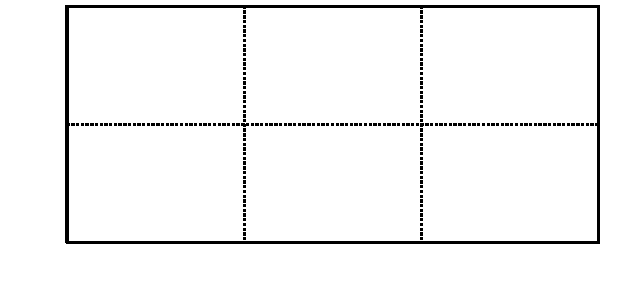
\includegraphics[width=0.6\linewidth]{Chapter_2/13}
    \caption{Схема для исследования затухания} \figmark{scheme damping}
\end{figure}

Амплитуда сигнала на выходе из волновода~$E$ убывает с пройденным 
расстоянием $z$ как $E=E_0e^{-\alpha z}$, где $E_0$~--- амплитуда входного
сигнала. Для мощности (интенсивности), пропорциональной квадрату амплитуды,
 имеем $W=W_0e^{-2\alpha z}$ или $W=W_0 10^{-\beta z}$,
где $\alpha = \beta \frac{\ln 10}{2} \approx 1{,}15 \beta$.
Ослабление интенсивности сигнала $\gamma=\beta z$ принято измерять в \emph{децибелах}~(дБ):
\[
\gamma \; [\text{дБ}] = 10 \lg \frac{W_0}{W},
\]
то есть 10~дБ соответствует уменьшению интенсивности (мощности) в~10~раз. Величину
$\alpha z=\ln \frac{E_0}{E}$ также иногда измеряют в \emph{неперах} (Нп):
ослабление на~1~Нп соответствует уменьшению амплитуды в~$e$ раз.
Нетрудно видеть, что 
$1\;\text{Нп} = \frac{20}{\ln 10}\;\text{дБ} \approx 8,69\;\text{дБ}$.

Если при уменьшении количества вставок волновода поддерживать интенсивность
выходного сигнала постоянной, то входной сигнал следует ослабить. Ослабление
$\beta z$ зависит от длины волновода $z$ и измеряется по шкале генератора в децибелах. 
Так в эксперименте определяется коэффициент~$\beta$. 
Его можно сравнить с коэффициентом $\alpha$, рассчитанным теоретически. 
В закритическом волноводе при квадратичном детектировании интенсивность сигнала 
падает по закону $U\propto E^2 \propto e^{-2\alpha z}$,
где $\alpha$~---~коэффициент затухания \chaptereqref{alpha}: 
\begin{equation} \eqmark{2.0.7}
\alpha=\frac{1}{c}\sqrt{\omega_{кр}^2-\omega^2}=
\dfrac{\pi}{a}\sqrt{1-\left(\dfrac{\lambda_{кр}}{\lambda_0}\right)^2}. 
\end{equation} 
Здесь $\lambda_0=c/\nu_0$~--- длина волны в свободном пространстве
при рабочей частоте $\nu_0$, и $\lambda_{кр}=2a$ --- критическая длина волны, $a$~--- размер широкой 
стенки волновода-вставки ($\nu_0$ и $a$ указаны в техническом описании установки).

\begin{lab:task}
    
    \taskpreamble{В работе предлагается при частоте выше критической исследовать
        стоячую волну в измерительной линии (рис.~\figref{scheme microwave}): измерив
        распределение сигнала вдоль волновода, рассчитать фазовую скорость; затем, меняя
        нагрузку на выходе волновода (заглушка, открытый конец или поглотитель),
        определить коэффициенты отражения волн $r$. При частоте ниже критической
        предлагается определить коэффициент затухания волны $\beta$ в сборном 
        волноводе (рис.~\figref{scheme damping}) и сравнить с его теоретическим значением.}
    
    \tasksection{А. Исследование структуры волн при частоте выше критической}
    
    \item Проведите подготовку приборов к работе по техническому описанию (ТО),
    лежащему на рабочем столе. Ознакомьтесь с расположением и назначением
    ручек регулировки приборов.
    
\begin{lab:warning}
Мощность сигнала, создаваемого с генератора, невелика, поэтому
    излучение не представляет опасности для здоровья человека. Тем не менее
    заглядывать в открытый волновод при включённом генераторе не рекомендуется!
\end{lab:warning}
    
    \tasksection{I. Определение длины волны СВЧ-сигнала в волноводе}
    
    
    
    \item Установите рабочую частоту $\nu_0$ (см. техническое описание установки); 
    перемещая зонд, настройтесь на пучность стоячей волны. 
    Если при этом показания вольтметра превышают 1~мВ, 
    следует с помощью аттенюатора ослабить сигнал, идущий от генератора  (при
    напряжениях $\ge1$~мВ меняется характер детектирования).
    
    \item Подберите чувствительность вольтметра так,
    чтобы в максимуме стрелка отклонялась почти на всю шкалу. Используя весь
    возможный диапазон перемещения зонда вдоль измерительной линии, измерьте
    зависимость показаний вольтметра~$U$ от положения зонда~$z$ (100 делений винта
    у выхода измерительной линии соответствуют 1~мм). Менять чувствительность
    вольтметра в течение этой серии нецелесообразно.
    
    \item Постройте график $U(z)$ и определите по нему длину волны
    $\lambda_{\text{в}}$ в волноводе. Сравните результат с теоретическим расчётом.
    Рассчитайте фазовую скорость $v_{\text{ф}}$ волн в волноводе. 
%    Рассчитайте групповую скорость $u,$ используя соотношение
%    $uV_{\text{Ф}}=c^2.$
    
    \tasksection{II. Определение коэффициентов отражения}
    
    \item Снимите металлическую заглушку с фланца измерительной линии. Перемещая
    зонд, измерьте максимальное ($U_{\text{max}}<1$~мВ) и минимальное напряжения
    в волне.
    
    \item Наденьте на выходной фланец измерительной линии отрезок волновода с
    поглощающей нагрузкой и снова измерьте максимальное и минимальное напряжения.
    
    \item Считая детектирование квадратичным, определите коэффициенты 
    отражения~$r$ для открытого и закрытого волновода и для волновода 
    с поглощающей нагрузкой. Объясните полученные результаты.
    
    \tasksection{Б. Исследование затухания волн при частоте ниже критической}
    
    \item Соберите схему согласно рис.~\figref{scheme damping} и настройте её по
    техническому описанию (ТО).
    
    \item Измерьте длину каждой волноводной секции.
    
    \item Используя размер $a$ широкой стенки волновода, указанный на установке,
    рассчитайте критическую частоту волновода $\nu_{кр}= \omega_{кр}/2\pi$. 
    Убедитесь, что рабочая частота~$\nu_0$ меньше критической.
    
    \tasksection{III. Измерение коэффициента затухания}
    
    \item Настройте детекторную головку на максимальную чувствительность согласно~ТО, 
    расположенному на установке (в этом упражнении ограничение $U<1$~мВ
    необязательно). Установите минимальное затухание ($\gamma=20$~дБ) сигнала от
    генератора и подберите чувствительность вольтметра так, чтобы стрелка
    отклонялась почти на всю шкалу; зарегистрируйте величины~$U$ и~$\gamma$.
    
    \item Последовательно уменьшая число промежуточных секций от трёх до нуля,
    каждый раз подбирайте такое ослабление сигнала от генератора, при котором
    показания вольтметра усилителя остаются неизменными.
    
    \item Постройте график в функции $\gamma(z),$ где $z$~---~полная длина
    подключённых волноводных секций. По наклону прямой рассчитайте коэффициент
    затухания $\beta=\frac{\Delta\gamma}{\Delta z}$ 
    в единицах $[\text{дБ}/\text{см}]$ и сравните результат с теоретическим
    расчётом \eqref{2.0.7}.
 \end{lab:task}


\begin{lab:questions} 
    
    \item Является ли электромагнитная волна в волноводе поперечной?
    
    \item Какие компоненты электрического и магнитного полей отличны от нуля
для основной моды $H_{10}$ в прямоугольном волноводе?

    \item Найдите распределение магнитного поля внутри волновода для моды $H_{10}$.

    \item Найдите минимальную частоту для $E$-волны в прямоугольном волноводе (волны с ненулевой
    продольной компонентой $E_z\ne 0$).
    
    \item Найдите критическую частоту и длину волны для моды $H_{nm}$ в прямоугольном волноводе.
    
    \item Используя выражения для групповой и фазовой
    скоростей $v_{гр}=d\omega/dk_z$, $v_{\text{ф}}=\omega/k_z$, покажите, что в
    волноводе справедливо $v_{гр}v_{\text{ф}}=c^2$.
    
    \item Как направлен вектор Пойнтинга в волноводе с идеально проводящими стенками?
\end{lab:questions}


\begin{lab:literature} 
    \item \Kirichenko~--- \S~13.2.
    
    \item \SivuhinIII~--- \S~139, 140.
    
    \item \KingLokOlh~--- Ч.~III. \S~6.7.
        
%    \item Фейнмановские лекции по физике. Т.~6. Электродинамика. – М.:~Наука, 1966,
%    гл.~24. 
\end{lab:literature}
